
\chapter{Literature study}
\label{chapter:title}
To get familiar with the concepts and questions that may arise during the design, a literature study was carried out. Various aspects (but not all) of the design are being explored here.
\section{Requirements for the bogie}\\ \\


This project will consist of different phases in order to come up with a test proposal for a rocker bogie design for a planetary rover vehicle for IAC (Important Aerospace Company). This chapter will elaborate on these phases.
For the design of the rocker bogie, the team will take basic engineering design steps following the DESACME/I process. The measures of this process are as follows:
First, the problem needs to be defined….. blabal SEE ADSEE PPT
Then Establish requirements
After establishing the requirements, the team will set up options. For this, previous approaches will be studied, even the ones without any success. 
Now it will be time to analyze the options set. This will be done with fundamental principles clear in mind. Nonetheless, there is no time and money to evaluate all the ideas in detail already. The level of analysis has to be sufficient to set up a fair trade off between the various concepts and select a preferred concept to proceed.
This is where comparing the options comes in play. A number of criteria must be identified and assigned appropriate weights to reflect the requirements initially agreed on with, in this case, IAC.
The next phase is making a choice. After weighing all the options and discussing the trade-offs, choosing an option is as important as difficult. 
Almost arriving at the end phase, the outcome has to be evaluated. The team will have to have a critical view on their own results in order to decide the next step and to report the work done.
If necessary, this engineering design cycle will be iterated to improve the final result. During this project however, there will be no time to go over all the steps again, but usually there are several iterations needed for the best result.
During the last phase, all the work done and methods used will be documented in a report of 15 to 20 pages.



It is rather hard to come up with a design without a goal so luckily, IAC has set a couple of requirements to be met for the rocker bogie design. The structure of the bogie has to be rigid, but due to the trustworthiness, a hinge is  installed at points A and B. This gives the rover bogie the ability to drive over the rocky terrains certain planets consist of. It should be capable of driving over obstacles of d_h= 70cm. IAC also demands the rover to drive with a velocity of v=0.085mph. The vehicle, also referred to as EDD-E, has two cameras on top 
The vehicle will be equipped with various measurement devices, each with their own internal system requirements. Having said that, one of the devices will be highlighted in this paragraph; a drill which can identify the type of soil by measuring the resistance on the drill bit. When drilling starts, the cross-beam hinge at point A in Figure … is locked. The drill, however, is attached to an arm on the frontside of the rover and will create a torque around the cross-beam which joins the rover’s body to both sides of the bogie system. To ensure the rover drills flawlessly vertical, the mentioned beam cannot twist more than theta=0.5deg at a torque of T=200Nm. 


\section{Understanding of the natural frequency}
To adjust our design to the given requirements, there has to be an understanding of the variable of natural frequency. The natural frequency itself is defined by many variables related to both the geometry and the material of a structure. The equation for the determination of the magnitude of the natural frequency is given by;
\begin{equation} \label{natural frequency, q2}
    f_n = \frac{1}{2\pi} \cdot \sqrt{\frac{k}{m}}
\end{equation}
Equation \eqref{natural frequency, q2} consists of the variables m (mass) and k. Here k is the 'stiffness' of the structure. The magnitude of this variable can be approached by dividing the force ($F$) by the accompanying deflection ($\delta$). Hence,
\begin{equation}
    k = \frac{F}{\delta}
\end{equation}
Also, $\delta$ can be defined by the following equation.
\begin{equation}
    \delta = \frac{F \cdot L^3}{48 \cdot E \cdot I}
\end{equation}
With F the force applied, L the length of the structure, E the Young's modulus and I the moment of inertia.
So concluding which variables/parameters govern the natural frequency of a structure, we see that there are two main pillars to which they do contribute. \\
\textbf{Geometry}
\begin{itemize}
    \item Lenght ($L$). This is obviously related to the geometry. \textit{The larger L, the smaller the natural frequency.}
    \item Moment of Inertia ($I$). This has to do with the geometry of the structure. Indirectly, the center of gravity (c.g.) depends the magnitude of I. In general, \textit{the farther away the c.g. is from the rotating axis, the larger the moment of inertia.} This is true when the considered structure is made of one single material.
\end{itemize}
\textbf{Material}
\begin{itemize}
    \item Mass ($m$). The magnitude depends on the density of the material and thus the mass is a mainly a material property.
    Of course, the mass could also be categorised in the geometry part (the volume used). \textit{The larger the mass, the smaller the natural frequency.}
    \item Young's modulus ($E$). Every type of material has a different Young's modulus. These typically range from $10^-4$ up to $10^3$ GPa. \textit{The larger the Young's modulus, the smaller the natural frequency.}
\end{itemize}
So concluding, the natural frequency of a structure depends on several (in)dependent properties which are either related to the choice of geometry or the choice of material.
\newline
Apart from the the vibrations in the structure, also the environment around the structure is important to make a well-considered choice regarding the material.
\section{Impact of the environment on the choice of material}
When the temperature of the atmosphere of the different planets increases, the stiffness of the material will decrease. This way, for planets with high temperatures we need materials with a high yield stress. Equally, when the temperature is really low, the material has a high change of cracking so we need a high fracture toughness.

When a planet has a high gravity constant, the gravity force of the rover will increase. By the formula 
\begin{equation} \sigma = \frac{F}{A}
\end{equation}
We can conclude that we need a higher stiffness for a bigger force, so we need a material with a high yield strength.
The change in design parameters also depends on the surface of the planet. When the surface has, for instance, a though surface with lots of rocks and dust, we need wheels with a lot of grip and high fracture toughness, so the wheels won't crack. 

When a planet has a lot of ultraviolet light from for example the sun or an other nearby star, there will occur UV degradation on the material. The absorbed energy can excite photons in plastic and these can create free radicals. In the presence of radical receptors on the planet, the material can crack. On planets with a lot of UV light, it is therefore best to not use plastic. Also high energy waves(radiation) can effect the materials and even the instruments of the rover, however this will only be a problem it there is a lack of atmosphere. This is a significant problem in environments like the Moon and Mars


-Atmospheric composition
Other planets bring different atmospheres, a consequence of a different atmosphere is that it can be a very hostile environment for the rover. As a result the composition of the atmosphere has to be accounted for. A atmosphere can contain different gasses that all have different effects on the materials of the rover. 
One form of corrosion is caused by oxygen that is dissolved in water, so if the atmosphere is very dry this will not be a problem but when the atmosphere is humid this could seriously affect the material by corrosion. 
Another form of corrosion is metal dusting. This occurs when there is a presence of carbon mono-oxide, however at temperatures below 300 degrees this is very insignificant only at very high temperatures above 300 degrees this rusting has to be taken in to account.
Some  metals such as stainless steel and aluminium alloys also rust in the presence of chloride but also in this case there has to be a presence of water. 
Corrosion rates are also very much influenced by conditions as humidity, temperatures and the presence of contaminants such as Chlorides. So when going on a mission to another planet this all has to be looked in to. Corrosion can be prevented by treating the metal or choosing a metal that won't easily corrode.



\section{Launch loads and vibrations}

Nowadays, many governments and companies produce rockets so there is a wide variety of data that all these rockets have. In order to calculate the expected launch loads on the Rocker Bogie a selection of 4 commonly-used rockets is made: Soyuz (Russia), Falcon 9 (SpaceX, USA), Ariane 5 (Europe) and Atlas 5 (USA).

\begin{figure}[h!]
\centering
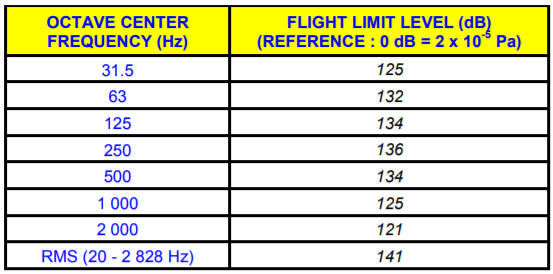
\includegraphics[width=8cm]{figures/Soyux_vibra.png}
\caption{Soyuz vibrations}
\label{Soyuz vibrations}
\end{figure}

\begin{figure}[h!]
\centering
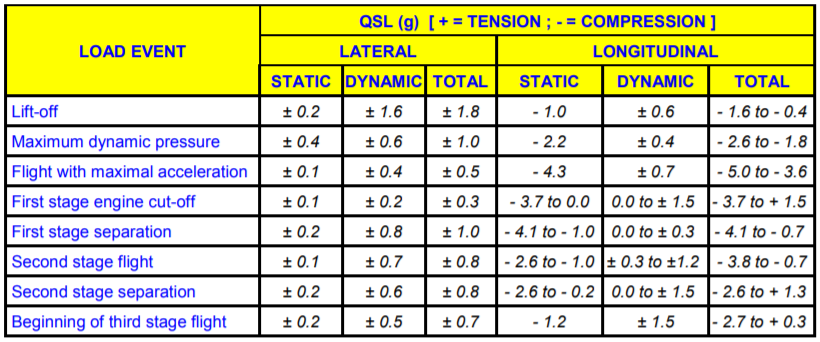
\includegraphics[width=8cm]{figures/Soyuz_acce.png}
\caption{Soyuz acceleration}
\label{Soyuz acceleration}
\end{figure}


\begin{figure}[h!]
\centering
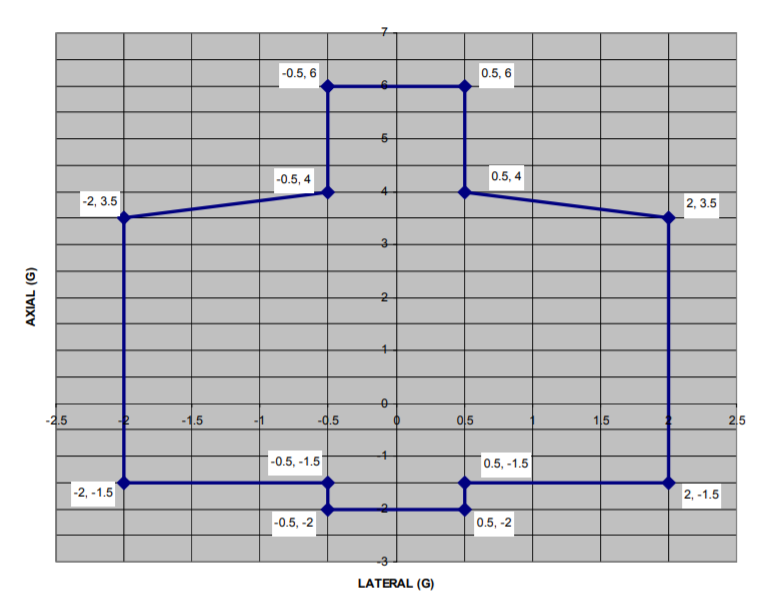
\includegraphics[width=8cm]{figures/Falcon9_acc.png}
\caption{Falcon 9 acceleration}
\label{Falcon 9 acceleration}
\end{figure}

\begin{figure}[h!]
\centering
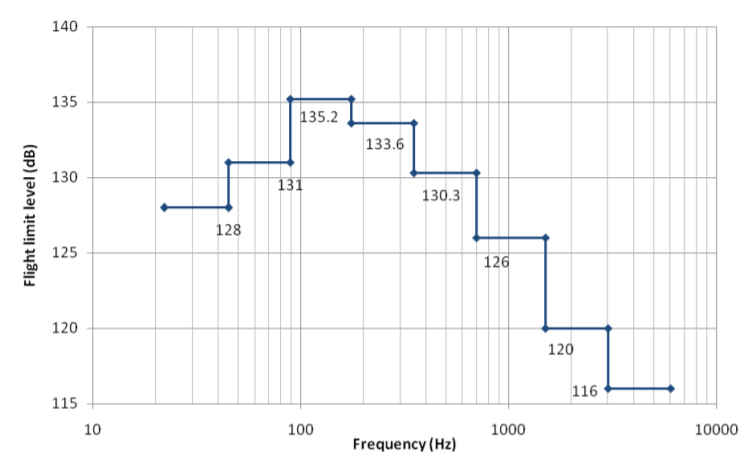
\includegraphics[width=8cm]{figures/Falcon9_vibr.png}
\caption{Falcon 9 vibrations}
\label{Falcon 9 vibrations}
\end{figure}

\clearpage

\begin{figure}[h!]
\centering
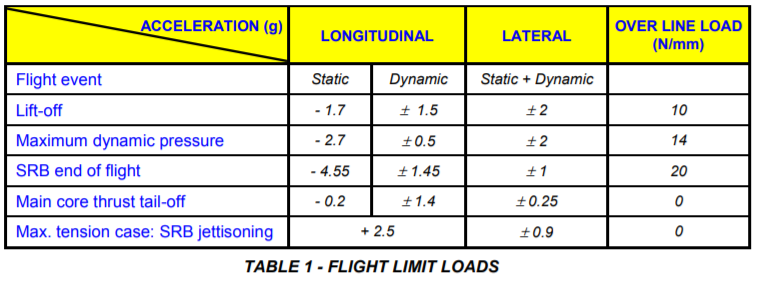
\includegraphics[width=8cm]{figures/Ariane5_acc.PNG}
\caption{Ariane 5 acceleration}
\label{Ariane 5 acceleration}
\end{figure}

\begin{figure}[h!]
\centering
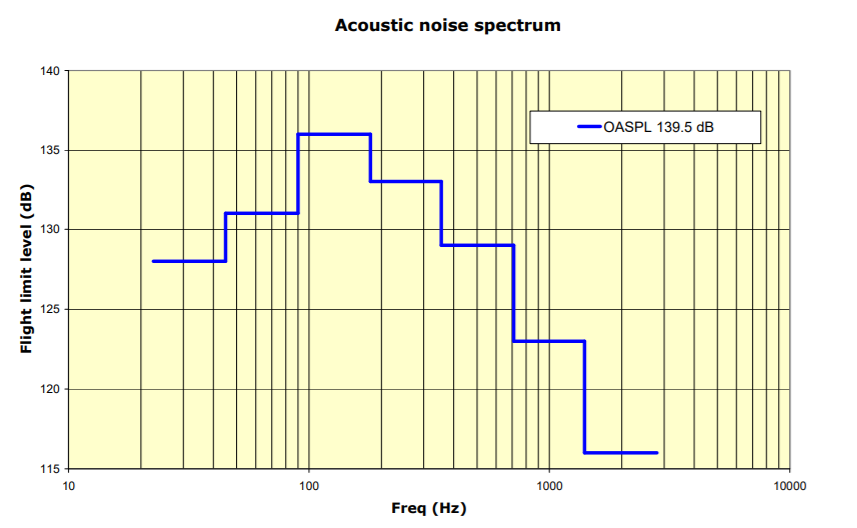
\includegraphics[width=8cm]{figures/Ariane5_Vibr.png}
\caption{Ariane 5 vibrations}
\label{Ariane 5 virbrations}
\end{figure}

\begin{figure}[h!]
\centering
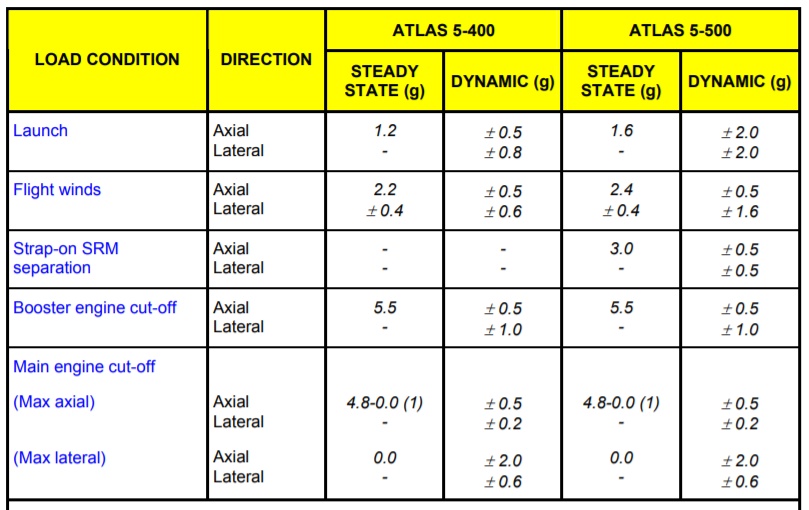
\includegraphics[width=8cm]{figures/Atlas5_acc.PNG}
\caption{Atlas 5 acceleration}
\label{Atlas 5 acceleration}
\end{figure}

\begin{figure}[h!]
\centering
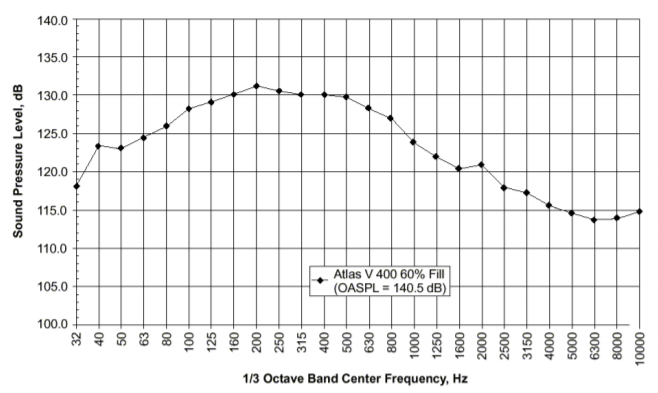
\includegraphics[width=8cm]{figures/Atlas5_vibr.PNG}
\caption{Atlas 5 vibrations}
\label{Atlas 5 virbrations}
\end{figure}

Considering all this data an assumption can be made about what launch loads the Rocker Bogie should withstand. By examining these examples we can conclude that generally the static loads are between 4-6g at peak loading which is at booster engine cut-off. At this peak loading the Rocker Bogie should be able to withstand a load 4 to 6 times its own weight relative to that on Earth.
\\

At the same time the Rocker Bogie should also coop with the frequencies released during flight. The spectrum of frequencies are shown in figures 2.1, 2.4, 2.6 and 2.8. Frequencies like these create stresses in the materials which can over time create fatigue loading.



\section{Question 6}

One of the main benefits of using composite structures in space environments is the relatively high specific strength and toughness compared to metals. This often allows a spacecraft containing a lot of composites to be less heavy than a spacecraft which is loaded in the same load cases but mostly consists of metal. Lower dry weight is important in spacecraft since it allows for higher performance. 

One big drawback of a lot of composite materials is the fact that they are highly anisotropic. Because of this, the strength might be high in the longitudinal direction while it’s very low in the transverse direction. During launch when most forces act in one direction it is less of a problem, but in general, it can be a bigger issue. This can be counteracted by applying fibers in all directions, but this will significantly lower the maximum strength which could defeat the purpose of using composites in the first place since metals are already isotropic. 

Another very important property of using composite materials especially in space environments is that they usually have allow coefficient of thermal expansion compared to metals. Volumatic expansion is given by the formula
\begin{equation}
    \frac{\Delta V}{V} = \alpha \cdot \Delta T
\end{equation}
Which says that with a low expansion ration the difference in volume will be smaller
This is very important since the temperature changes in space are often very high. The temperatures of the moon, for instance, can vary between day and nighttime with as much as 290 degrees Kelvin. Since the expansion coefficient for metals is significantly higher with high coefficients will expand more, risking damage to the structure. This does however heavily depend on the composite used since the matrix and the fiber can have a different expansion coefficient which could do damage to the composite itself when the fiber separates from the matrix. 

A big downside of using composite materials is that the plastic matrix will be eroded due to the UV radiation, therefore it is better to use metals in environments with high levels of UV radiation. In space environments, there is no magnetosphere or a thick atmosphere to protect from the harsh UV radiation from the sun. Because of this, the composite materials with a plastic matrix will degrade faster then they would on earth. 

Another negative is the relatively high price of production of composite materials compared to most metals. The use of a lot of composite materials can, therefore, drive up the costs of a mission or take away funds from different aspects of the mission.

\section{Question 7}
The bending stiffness of a beam (EI), can be derived from the formula of the spring constant in lateral direction.
\begin{equation}
    k_y= \frac{3EI}{L^3}
\end{equation}
This formula can be rewritten in the form:
\begin{equation}
    EI=\frac{L^3 \cdot k_y}{3}
\end{equation}
Where L is the length of the beam and $k_y$ is the spring constant. With this formula you can calculate the bending stiffness of a aluminium beam. The formula for a fully composite beam can be obtained as\cite{Composite-beams}
\begin{equation}
    EI= EI_0 + \frac{EA_p \cdot r^2}{EA_0}
\end{equation}
where $AE_p$ is the product of axial stiffness of subelements, $AE_0$ is the sum of axial stiffness of the subelements and $EI_0$ is the bending stiffness of noncomposite section given by
\begin{equation}
    EI_0=-\frac{M}{w}
\end{equation}
where M is the internal moment and w is the displacement in the z-direction.
The torsional stiffness (GJ) for both a aluminium beam and a composite beam can be calculated with
\begin{equation}
    GJ = \frac{T\cdot L}{\Theta}
\end{equation}

\section{Question 8}

The structure of the rocker bogie has to withstand dynamic loads, such as heavy vibrations, during launch. After landing the vertical beams in the structure as can be seen in figure \ref{rockerbogiesketch} are loaded in compression and the horizontal ones in bending as it supports the weight of rest of the vehicle. Whilst withstanding the different load cases, EDD*E, the universal planet reconnaissance vehicle which the rocker bogie structure supports, must properly function during operation on different planetary surfaces with different environmental conditions.
\\
\\
\begin{figure}
    \centering
    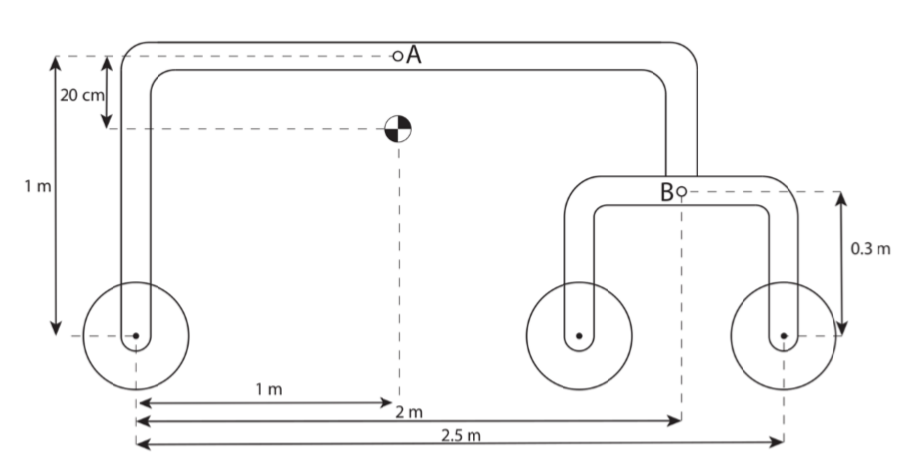
\includegraphics[width=8cm]{figures/Rockerbogiesketch.png}
    \caption{Rocker bogie beams sketch from \cite{project-manual}}
    \label{rockerbogiesketch}
\end{figure}
\\
\\
As is described in \cite{alderliesten-introduction-to-aerospace-structures-and-materials}, when analysing the primary loads during launch, most will largely be of influence on the launch vehicle, not the payload. The payload, in this case EDD*E, will however be subject to quite severe vibrations. Cyclic loading such as this can result in failure, usually in the form of fatigue damage. Metals such as aluminium initially respond to vibrations by strain hardening, increasing the strength of the material. It takes long for cracks to propagate and reach a critical crack length as is described in \cite{ashby-aerospace-materials}. Strain hardening in composites is negligible making the phase in which the crack propagates much shorter than for aluminium. Once sufficient damage is available in the material, it progresses to failure fairly quickly. On the other hand, composites do offer certain vibration damping properties which, in one way, can be achieved by the addition of vibration damping material as is described in \cite{Sound-and-vibration-damping}. Even though it solves the vibration problem, these processes do add weight to the final structure and are expansive to manufacture. 
\\
\\
Another danger of the vibrations during launch is if the rocker bogie structure were to approach its natural frequency. Oscillations increase drastically if that were to happen. To ensure the safety of the rocker bogie, its natural frequency should be well above the frequency of the vibrations caused by the launch vehicle. As given in \cite{Introduction-to-Aerospace-Structures-and-Materials} the equation for the natural frequency of a mass spring system is the following:
\\
\\
\begin{equation} \label{naturalfreq}
    f_n= \frac{1}{2\pi} \cdot \sqrt{\frac{k}{m}}
\end{equation}
\\
\\ 
Equation \ref{naturalfreq} shows that the natural frequencies can be increased by decreasing the mass of the structure. Composites generally have lower densities than aluminium alloys as can be seen in figure \ref{bubblechart}.
\\
\\
\begin{figure}
    \centering
    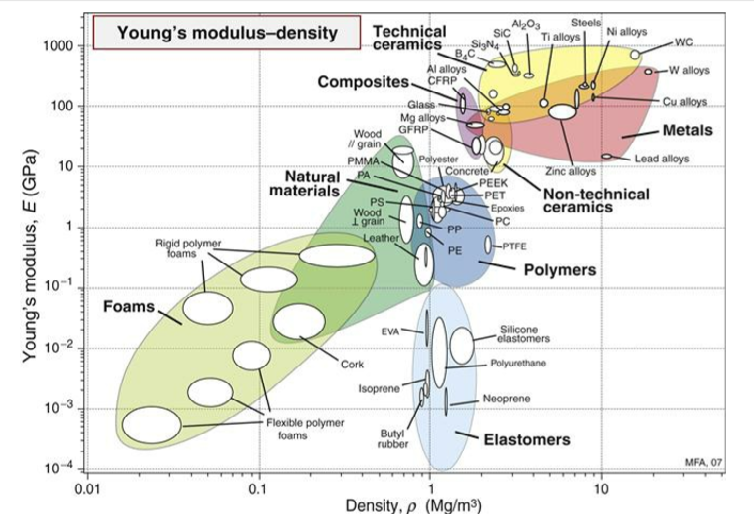
\includegraphics[width=8cm]{figures/Bubble chart.png}
    \caption{Elastic modulus-Density bubble chart \cite{ashby-aerospace-materials}}
    \label{bubblechart}
\end{figure}
\\
\\
Assuming the dimensions of the structure will remain about the same, regardless of which material is used. A structure made out of composites would have a lower mass and thus a higher and safer natural frequency. The structure can however be designed properly so as to stay in a safe range of frequencies even when using the heavier aluminium.
\\
\\
A higher mass decreases the natural frequency. This shows a part of the general main objective in aerospace design of the minimization of weight. A part of weight minimization comes from the objective of cost minimization. A lighter structure of the same material means saving up on material costs, since less is needed to produce the structure. Composites have a very positive stiffness-to-weight ratio, considerably better than aluminium. For the same required stiffness, composite structures are lighter than aluminium, an obvious advantage. Opposite of that composites do have high production costs considering that the production is very complicated and labour-intensive. Aluminium however, has great manufacturability. It’s quite cheap and easy to apply production processes like forming or machining. Even though composites do have adequate workshop properties, they get much harder to cut by machining when the strength of e.g. the fibres increases. To be able to machine composites, the strength is partially sacrificed by using weaker fibres, which is an undesirable result.
\\
\\
On another note; after EDD*E has landed on a planetary surface it is more prominently subjected to different loading cases. The simple design of the rocker bogie structure consists of multiple beams mostly loaded in either compression (The vertical beams) or bending (The horizontal beams). By placing a hinge at both positions A and B as shown in figure \ref{rockerbogiesketch}, the bending loads in the horizontal beams are partially prevented leaving the most prominent loading case to be the compression in the vertical beams. Composites are anisotropic and even though they’re a great choice for when the main load case is uniaxial tension, they’re not ideal when loaded in compression. Aluminium is isotropic, it can be loaded in any direction and has similar strength in both tension and compression. Therefore compressive loads, as present in part of the rocker bogie structure, can have destructive results when it’s made out of composites whilst it will generally lead to very little to no damage in metals such as aluminium.
\\
\\
For EDD*E to be able to function properly on different planetary surfaces, the conditions in which it has to operate can differ greatly. The structure of the rocker bogie is required to withstand certain loads during operation, specific operating conditions can negatively influence the structures properties, e.g. reducing the strength of the material. 
\\
\\
The possible operating conditions on the different planetary surfaces may include a large range of temperatures in which it must be able to operate. All engineering materials, thus including both composites and aluminium, show some temperature dependent behaviour. An increase in temperature often leads to material properties deteriorating. The range of safe operating temperatures are influenced by many different factors and both aluminium and composites can be modelled towards a positive operating temperature window.
\\
\\
As can be read in \cite{thermal-properties-aluminium} the properties of aluminium don’t change as drastically as some other materials when it undergoes a change in temperature. Aluminium has no ductile-to-brittle transition, therefore it stays tough even at lower temperatures leading up to almost  -200 degrees Celsius (cryogenic). As the temperature increases, aluminium doesn’t intrinsically keep it’s strength, but by using methods such as solid-solution strengthening, second phase hardening and the use of rapid solidification technology, there is the possibility to create aluminium that show promise for operating at temperatures up to 350 degrees Celsius.
\\
\\
Composites, however, show much more drastic changes in their properties as the temperature is either increased or decreased as is described in \cite{Thermal-behaviour-of-composites}. Considering that composites are made of multiple different materials, these all show a different reaction to the temperature change. The materials will either contract or expand which results in internal stresses and even a separation of the reinforcement and matrix e.g. delamination \cite{Thermomechanical-behaviour-of-composite-materials}.
\\
\\
Aside from the temperature changes, there is also the possibility of an aggressive environment in which EDD*E must properly operate without having some form of degradation leading to failure of the rocker bogie. Both aluminium and composites are generally not resistant to oxidation, but could be protected by using for example a coating to protect the material from the possibly hostile environment. Where aluminium has a real advantage however is that when it oxidizes, it actually forms a protective oxide film. This film protects the surface, which it strongly adheres to, against corrosion.
\\
\\
In conclusion, even though composites are the obvious candidate in certain aspects of the design, the properties of aluminium ultimately exceed them. It is more cost-effective to make the structure out of aluminium and it shows more promising properties to withstand the loading cases after landing and the planetary conditions. Aluminium is ultimately the safer choice.



